\documentclass[sigconf]{acmart}
\usepackage{cleveref}
\usepackage{graphics}
\settopmatter{printacmref=false}
\setcopyright{none}
\renewcommand\footnotetextcopyrightpermission[1]{}
\pagestyle{plain}
\crefformat{section}{\S#2#1#3}

\definecolor{codegreen}{rgb}{0,0.6,0}
\definecolor{codegray}{rgb}{0.5,0.5,0.5}
\definecolor{codepurple}{rgb}{0.58,0,0.82}
\definecolor{backcolour}{rgb}{0.95,0.95,0.92}

\usepackage{listings}
\usepackage{xcolor}
\usepackage{upquote}

%New colors defined below
\definecolor{codegreen}{rgb}{0,0.6,0}
\definecolor{codegray}{rgb}{0.5,0.5,0.5}
\definecolor{codepurple}{rgb}{0.58,0,0.82}
\definecolor{backcolour}{rgb}{0.95,0.95,0.92}

%Code listing style named "mystyle"
\lstdefinestyle{mystyle}{
  backgroundcolor=\color{backcolour},   commentstyle=\color{codegreen},
  keywordstyle=\color{magenta},
  numberstyle=\tiny\color{codegray},
  stringstyle=\color{codepurple},
  basicstyle=\ttfamily\footnotesize,
  breakatwhitespace=false,         
  breaklines=true,                 
  captionpos=b,                    
  keepspaces=true,                 
  numbers=left,                    
  numbersep=5pt,                  
  showspaces=false,                
  showstringspaces=false,
  showtabs=false,                  
  tabsize=2,
  keepspaces=true,
  language=java, 
  moredelim=[is][\underbar]{_}{_}
}

\lstset{style=mystyle}


\usepackage[most]{tcolorbox}

%textmarker style from colorbox doc
\tcbset{textmarker/.style={%
        enhanced,
        parbox=false,boxrule=0mm,boxsep=0mm,arc=0mm,
        outer arc=0mm,left=6mm,right=3mm,top=7pt,bottom=7pt,
        toptitle=1mm,bottomtitle=1mm,oversize}}


% define new colorboxes
\newtcolorbox{hintBox}{textmarker,
    borderline west={6pt}{0pt}{yellow},
    colback=yellow!10!white}
\newtcolorbox{importantBox}{textmarker,
    borderline west={6pt}{0pt}{red},
    colback=red!10!white}
\newtcolorbox{noteBox}{textmarker,
    borderline west={6pt}{0pt}{green},
    colback=green!10!white}

% define commands for easy access
\newcommand{\note}[1]{\begin{noteBox} \textbf{Note:} #1 \end{noteBox}}
\newcommand{\warning}[1]{\begin{hintBox} \textbf{Warning:} #1 \end{hintBox}}
\newcommand{\important}[1]{\begin{importantBox} \textbf{Important:} #1 \end{importantBox}}



\begin{document}
%%
%% The "title" command has an optional parameter,
%% allowing the author to define a "short title" to be used in page headers.
\title{Suggesting Secure Implementation to Vulnerable Code Snippets on Stackoverflow.}


\maketitle
\section{Introduction}
\begin{lstlisting}[caption={A real code snippet taken from Stackoverflow. I want to build a tool which after analyzing the code snippet will highlight the part of the code that is insecure and suggest an alternative secure implementation as showed in the figure.}, label={fig:motivating-example}]
 private byte[] encrypt(byte[] raw, byte[] clear) {
   ...
   _Cipher cipher = Cipher.getInstance("AES")_;}
   // Cipher cipher = Cipher.getInstance("AES/CBC/PKCS5Padding");
   ....
   return encrypted
 }
  \end{lstlisting}
\label{into}
%\textcolor{blue}{we can't also using testing to test the code snippet mention it somewhere...}
%\note{Certainly elsewhere my do allowance at. The address farther six hearted hundred towards husband. Strangers ye to he sometimes propriety in. She right plate seven has. Bed who perceive judgment did marianne.}
In this project I want build a static analysis tool which will achieve the following. 
\begin{itemize}
\item  Analyze the code snippets from Stackoverflow for identifying out which part of the code is vulnerable by showing warning signs to highlight that part of the code to the developer.
\item When developer clicks on the warning sign a secure implementation while be shown to the developers. In case of failure of building generating a secure implementation, the tool will show insightful/helpful messages explaing why this part of the code is flaged as insecure.  
\end{itemize}

\section{Why the problem is interesting}
The problem is interesting for two reasons. 

\paragraph{Difficulty of writing crypto code securely.} Writing/implementing cypto code securely is a diffculut task for programmers. Any potential bug in crypto code can lead to serious vulnerablities open for attackers.
Even so unlike other code, crypto code can be insecure even if it works 
perfectly on traditional test-suite's input/output which is used only to prove the implementation correctness of the program.

\paragraph{Online platforms roles in spreading insecure code.} Online programming discussion platforms such as Stack Overflow have a rich source of ready to use code snippets for software developers. It is the defac-to place where developers go to find solutions of their problems and turn to the community for answers to their problems. 
Insecure code snippets found on Stackoverflow itself is not a serious problem. However,  
Fischer et al. has shown that developers have a tendency to directly copy paste code form Stack Overflow~\cite{fischer2017stack}. Therefore there are chances that any insecure code snippets posted on Stackoverflow can potentially find it way into production level code. To make matters worse, Meng et al.~\cite{meng2018secure} has showed that many accepted answers on Stackoverflow have seriously insecure code and often-times given by users having high reputation. This adds to the problem copy pasting vulnerable code from online platform and furthermore increases the chances of the insecure code snippet being trickled down to production level code. 
Unfortunately there is not state-of-the-art tool to analyzie if a code posted by developer on Stackoverflow is secure or not. In absense of such tool, Stackoverflow is potentially contributing as a major source of vulnerability in production level code.  

A static tool which can identify which part of the code snippet is insecure and suggest secure alternatives can help stopping the flow of insecure code from Stackoverflow to production level code.
\begin{figure}
  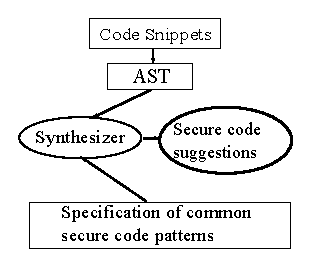
\includegraphics[width=0.5\linewidth]{Figures/workflow.eps}
  \caption{Proposed Methodology \textcolor{blue}{(Redraw the figure)}}
\end{figure}
\section{Proposed Methodology/Milestones}
As of now I am not really sure how to achieve the proposed goals described in \cref{into}. Especially how state-of-the-art synthesis techniques (e.g., program sketching) can be useful. However I am confortable analyzing insecurity of crypto code and therefore proposing the following methodology. 

My main idea is to convert the insecure and secure code snippets to AST and then apply synthesis to convert the insecure AST to secure AST \textit{somehow}. Again I am not sure about this synthesis part.  

\subsection{Data Collection \textcolor{blue}{(completed)}} 
I have collected code snippets of Stackoverflow from two existing sources. They are analyzed in ~\cite{fischer2017stack, meng2018secure} and publicy avaialble. 
They contain insecure code snippets of Java and Andrioid. 

I have compiled and arranged the coee snippets from two sources here \footnote{https://github.com/islamazhar/CS-703-Project/tree/master/insecure-code}. In future stages of the project I will add insecure codes from other languages as well using Stackoverflow's API.

\subsection{Identify Insecure Code Patterns \textcolor{blue}{(completed)}}
I have manually analyzed the insecure code in ~\cite{fischer2017stack,meng2018secure}. I have identified around 10 common insecure patterns which are most frequently occuring in them to an idea how secure code should look like. These 8 insecure partterns are briefly presented in Table.~\ref{tab:insecure-pattern}.
\iffalse
  \begin{figure*}[ht]
      \resizebox{\textwidth}{!}{
    \begin{tabular}{| l |l | l| l| l | l}
      \toprule
      No & Vulnerable insecure pattern &  Attack vectors & Crypto-property & severity & Way to secure \\
      \midrule
      1 & AES default encryption mode ECB which is vulnerable to side channel attacks & & & Using CBC encryption mode\\ 
      2 & Accetping all certificates in TrustManager by  implementing empty methods & & & Accepting only those certs which are in the trust chain \\ 
      3 & IV/Keys lacking randomn seed & & & IV/keys' seed should be generated from pesudo random functions\\
      4 & Keys having weak lengths & & & Using keys' having sufficient large length \\ 
      5 & Turing off CSRF protection & & & Do not turn of CSRF protection\\ 
      6 & Hard coded simple keys & & & Avoid using simple hard coded secret keys\\ 
      7 & Using Broken HASH MD5 & & & Avoid using broken hash MD5\\
      8 & Using insecure HTTP & & & Mandating usage of HTTPS\\ 
      \bottomrule
    \end{tabular}
      }
    \caption{Common insecure pattern and ways to secure them.}
    \label{tab:insecure-pattern}
  \end{figure*}
\fi
% Please add the following required packages to your document preamble:
% \usepackage{booktabs}
\iffalse
\begin{table*}[t]
  \begin{tabular}{|l|l|l|}
    \hline
    \begin{tabular}[c]{@{}l@{}}Rule\\ No\end{tabular} & Description                                  & Vulnerability                                             \\ \hline
    1                                                 & AES default encryption mode ECB              & Side channel attack                                       \\ \hline
    2                                                 & Insecure cryptographic hash                  & Collision attack                                          \\ \hline
    3                                                 & Presence of AllHostNameVerifier              & \multicolumn{1}{c|}{\multirow{3}{*}{SSL/TLS MitM attack}} \\ \cline{1-2}
    4                                                 & Abuse of X509TrustManager Verifier Interface & \multicolumn{1}{c|}{}                                     \\ \cline{1-2}
    5                                                 & Absence of performing hostname verification  & \multicolumn{1}{c|}{}                                     \\ \hline
    6                                                 & Weak key length                              & Brute force attack                                        \\ \hline
    7                                                 & Static/constant/predictable keys/IV          &                                                           \\ \hline
    8                                                 & Turning of CSRF protection                   & CSRF attack                                               \\ \hline    
    \end{tabular}
  \end{table*}
\fi
\textcolor{blue}{Ways to secure make a different table and mention the source where you are getting this secure implementaton...}
\subsection{Converting Code Snippets to AST \textcolor{blue}{(completed for rule 1)}}
\textcolor{blue}{
To analyze the code snippets for finding insecure parrterns, I have to convert these code snippets to Abstratc Syntax Tree (AST). However these code snippets are partially complete (i.e., missing classes, method implementations). Hence I have used a static analysis tool for partial java programs named PPA~\cite{dagenais2008enabling} to convert the code snippet to an intermidate representation Jimple.}

\textcolor{blue}{
Jimple~\cite{vallee1998jimple} is a 3-address intermediate representation that has been designed to simplify analysis. Jimple was inspired from SIMPLE an AST to represent C statements. 
We can feed the Jimple representation of the code snippet to soot -- a state-of-the-art we can traverse the jimple code to generate AST. 
}

\textcolor{blue}{
Each node (unit) of the generated AST from jimple representation consists of  around ~30 types of Stmt or Inst\footnote{https://www.sable.mcgill.ca/soot/doc/soot/Unit.html} -- which are in the grammer of Jimple. This Stmt or Inst are basically single/multiple line of code fragment from the code snippets. Now the problem simplifies to extracting those Stmt or Inst which are insecure.}

\subsubsection{Experiments}

\textcolor{blue}{For now I am currently focused on the rule no 1 (as shown on Table~\ref{tab:insecure-pattern}). This rule says that using default encryption mode ECB for AES encryption is vulnerable to side channel attacks. To prevent this we need to specify the a secure mode of the AES encryption (e.g., CBC, CFB, OFB, CTR). So we are searching for such nodes (units) in AST which has a statements such as \texttt{Cipher encipher = Cipher.getInstance("AES");} and want to replac them with a secure encryption mode such as \texttt{Cipher cipher = Cipher.getInstance("AES/CFB/NoPadding");}. This is code fragment is represented as a \texttt{InvokeStmt} class in Jimple. Therefore I am extracting those \texttt{InvokeStmt} and if the arguments passed to the invoke function is simply \texttt{AES} (i.e., insecure default mode of encryption), I identify them as insecure pattern. Currently I am justing showing a warning message with the line number saying 
\textit{``Use of default encryption mode in AES is vulnerable to side channel attacks. Consider using CBC/CFB encryption mode in line \#x".}}


\textcolor {blue}{I have analyzed first 30 insecure and secure code snippets related to rule 1 from the dataset which has a total of 1.3K code snippets. Among 12 code snippets which has the insecure parrtern, I can detect 5 of them. For the other 7 which I am unable to detect, they are either failing to produce the Jimple representation of those code snipeets as PPA is throwing exceptions or the default mode is passed as a constant. My implemenetation is currently conservative implying it does not produce warning when it can find the exact patterns I am looking for.}


\iffalse
\textcolor{blue}{
  Draw some code and their AST in the Appendix. Write the conversion part in details.
}
Next, I am planning to convert the secure and insecure implementation to abstract syntax tree (AST) for comparing. This can be difficult since these code snippets are partially complete (i.e., missing classes, method implementations). However Fischer et al.~\cite{fischer2017stack} have done it by integrating partial program analysis (PPA) tool~\cite{dagenais2008enabling} with WALA\footnote{https://github.com/wala/WALA}. However how they have done it, is not explained by Fisher et al. in details. I have experiences using PPA~\cite{dagenais2008enabling}. However I am familiar with PPA, but have not used WALA yet. %I am thinking about emailing the authors if the proposed methodology is approved by you. 

 I have generated AST of the code snippets using PPA. However PPA does not consider anonymous methods and as a result I have failed to generate AST for several code snippets.
\fi 
\subsection{Comparing AST of secure and insecure code / Repairing insecure AST from secure AST examples \textcolor{blue}{(incomplete)}}
\textcolor{blue}{
I am currently focused on implementation of detecting the other 7 rules. This would be challenging as they are staightforward as rule 1. For example, rule no 2 have anonymous class and as far as I know Jimple code does not support  anonymous class which can be a big problem. I am also going through the dataset of insecure code snippets to understand how the same insecure pattern is written in different ways by developers.} 

\textcolor{blue}{
I have read the paper which you have suggested~\cite{rolim2018learning}. This paper seems really relevent to the project. The difference is that we already have the quick fixes and do not need to learn them. Modifying the AST does seem co-related with what the project proposes. I will follow up with some updates on Monday office hour.}

\iffalse
\textcolor{blue}{Read the learning from quick fixes paper.}

This is the part I am mosting unsure of. I think synthesis will come handy here. 
I think the proper way should be finding the minimum changes we need to have to conver the AST built from insecure code to AST built from insecure code.  

If I can write first-order-logic for finding these minimum changes then that would be great. Because then I can use SMT solvers like Z3 to solve the constraints problem. 
So far I been unable to make progress in this direction and could not design the behavior constraints, structural constraints, and constraint solving part of the problem. I am also not sure how synthesis guided neural network can be useful or not. 

I have tried to go through the three papers on synthesis on the reading list of this course to get familiar with state-of-the-art techniques on program synthesis. I have some intuition. For example, repairing programs under uncertainty can be useful to synthesize code which needs to have IV/keys random with high entropy ~\cite{albarghouthi2017repairing}. Also I think Program sketching can be useful by placing holes in places where a cipher mode is used and writing assertion that any insecure ciphers can not used to fill up the hole.    

\section{Chanllenges}
I can think of the following challenges, I need to take care of while building the static tool.
\begin{itemize}
  \item The developed static tool needs to fast as if any developers post an insecure code it should not take much time to inform him/her that the code is not secure and where the problem is.
  \item It should not be too conservative (i.e, have low recall) and the same time high precision. Low recall will mean the static tool will always complain about the code snippet even if it is secure. Low precision means it will miss many of the insecure code snippets. We high precision and recall. 
\end{itemize}

\section{TODO list}
\textcolor{blue}{
\begin{itemize}
  \item Understanding the structure of vulnerable AST one by one for each rule presented in Table~\ref{tab:insecure-pattern}.
  \item How to repair the vulnerable AST and synthesize secure suggestions. 
  \item Testing the solution on the collected datasets.
\end{itemize}
%\section{Related work}
}
\fi
\section{Related work}
\section{Future work and limitations}

\bibliographystyle{ACM-Reference-Format}
  \bibliography{references}
  
%\section{Appendix}

% evalutation plan on datasets.
\end{document}
\end{document}